\documentclass[twoside]{book}

% Packages required by doxygen
\usepackage{fixltx2e}
\usepackage{calc}
\usepackage{doxygen}
\usepackage[export]{adjustbox} % also loads graphicx
\usepackage{graphicx}
\usepackage[utf8]{inputenc}
\usepackage{makeidx}
\usepackage{multicol}
\usepackage{multirow}
\PassOptionsToPackage{warn}{textcomp}
\usepackage{textcomp}
\usepackage[nointegrals]{wasysym}
\usepackage[table]{xcolor}

% Font selection
\usepackage[T1]{fontenc}
\usepackage[scaled=.90]{helvet}
\usepackage{courier}
\usepackage{amssymb}
\usepackage{sectsty}
\renewcommand{\familydefault}{\sfdefault}
\allsectionsfont{%
  \fontseries{bc}\selectfont%
  \color{darkgray}%
}
\renewcommand{\DoxyLabelFont}{%
  \fontseries{bc}\selectfont%
  \color{darkgray}%
}
\newcommand{\+}{\discretionary{\mbox{\scriptsize$\hookleftarrow$}}{}{}}

% Page & text layout
\usepackage{geometry}
\geometry{%
  a4paper,%
  top=2.5cm,%
  bottom=2.5cm,%
  left=2.5cm,%
  right=2.5cm%
}
\tolerance=750
\hfuzz=15pt
\hbadness=750
\setlength{\emergencystretch}{15pt}
\setlength{\parindent}{0cm}
\setlength{\parskip}{3ex plus 2ex minus 2ex}
\makeatletter
\renewcommand{\paragraph}{%
  \@startsection{paragraph}{4}{0ex}{-1.0ex}{1.0ex}{%
    \normalfont\normalsize\bfseries\SS@parafont%
  }%
}
\renewcommand{\subparagraph}{%
  \@startsection{subparagraph}{5}{0ex}{-1.0ex}{1.0ex}{%
    \normalfont\normalsize\bfseries\SS@subparafont%
  }%
}
\makeatother

% Headers & footers
\usepackage{fancyhdr}
\pagestyle{fancyplain}
\fancyhead[LE]{\fancyplain{}{\bfseries\thepage}}
\fancyhead[CE]{\fancyplain{}{}}
\fancyhead[RE]{\fancyplain{}{\bfseries\leftmark}}
\fancyhead[LO]{\fancyplain{}{\bfseries\rightmark}}
\fancyhead[CO]{\fancyplain{}{}}
\fancyhead[RO]{\fancyplain{}{\bfseries\thepage}}
\fancyfoot[LE]{\fancyplain{}{}}
\fancyfoot[CE]{\fancyplain{}{}}
\fancyfoot[RE]{\fancyplain{}{\bfseries\scriptsize Generated by Doxygen }}
\fancyfoot[LO]{\fancyplain{}{\bfseries\scriptsize Generated by Doxygen }}
\fancyfoot[CO]{\fancyplain{}{}}
\fancyfoot[RO]{\fancyplain{}{}}
\renewcommand{\footrulewidth}{0.4pt}
\renewcommand{\chaptermark}[1]{%
  \markboth{#1}{}%
}
\renewcommand{\sectionmark}[1]{%
  \markright{\thesection\ #1}%
}

% Indices & bibliography
\usepackage{natbib}
\usepackage[titles]{tocloft}
\setcounter{tocdepth}{3}
\setcounter{secnumdepth}{5}
\makeindex

% Hyperlinks (required, but should be loaded last)
\usepackage{ifpdf}
\ifpdf
  \usepackage[pdftex,pagebackref=true]{hyperref}
\else
  \usepackage[ps2pdf,pagebackref=true]{hyperref}
\fi
\hypersetup{%
  colorlinks=true,%
  linkcolor=blue,%
  citecolor=blue,%
  unicode%
}

% Custom commands
\newcommand{\clearemptydoublepage}{%
  \newpage{\pagestyle{empty}\cleardoublepage}%
}

\usepackage{caption}
\captionsetup{labelsep=space,justification=centering,font={bf},singlelinecheck=off,skip=4pt,position=top}

%===== C O N T E N T S =====

\begin{document}

% Titlepage & ToC
\hypersetup{pageanchor=false,
             bookmarksnumbered=true,
             pdfencoding=unicode
            }
\pagenumbering{alph}
\begin{titlepage}
\vspace*{7cm}
\begin{center}%
{\Large Tetris }\\
\vspace*{1cm}
{\large Generated by Doxygen 1.8.13}\\
\end{center}
\end{titlepage}
\clearemptydoublepage
\pagenumbering{roman}
\tableofcontents
\clearemptydoublepage
\pagenumbering{arabic}
\hypersetup{pageanchor=true}

%--- Begin generated contents ---
\chapter{Tetris}
\label{md__r_e_a_d_m_e}
\Hypertarget{md__r_e_a_d_m_e}
\hyperlink{class_jeu}{Jeu} Tetris à développer Librairies à télécharger \+:
\begin{DoxyItemize}
\item ncurses
\end{DoxyItemize}

Pour compiler le programme \+: g++ main.\+cpp -\/lncurses 
\chapter{Bug List}
\label{bug}
\Hypertarget{bug}

\begin{DoxyRefList}
\item[\label{bug__bug000001}%
\Hypertarget{bug__bug000001}%
Class \hyperlink{class_jeu}{Jeu} ]Rien à signaler 
\end{DoxyRefList}
\chapter{Hierarchical Index}
\section{Class Hierarchy}
This inheritance list is sorted roughly, but not completely, alphabetically\+:\begin{DoxyCompactList}
\item \contentsline{section}{Bloc}{\pageref{classBloc}}{}
\item \contentsline{section}{Board}{\pageref{classBoard}}{}
\item \contentsline{section}{I\+HM}{\pageref{classIHM}}{}
\item \contentsline{section}{Jeu}{\pageref{classJeu}}{}
\begin{DoxyCompactList}
\item \contentsline{section}{Jeu\+Classique}{\pageref{classJeuClassique}}{}
\item \contentsline{section}{Jeu\+Montagnard}{\pageref{classJeuMontagnard}}{}
\end{DoxyCompactList}
\item \contentsline{section}{Personnage}{\pageref{classPersonnage}}{}
\item \contentsline{section}{Piece}{\pageref{classPiece}}{}
\begin{DoxyCompactList}
\item \contentsline{section}{Piece\+\_\+I}{\pageref{classPiece__I}}{}
\item \contentsline{section}{Piece\+\_\+J}{\pageref{classPiece__J}}{}
\item \contentsline{section}{Piece\+\_\+L}{\pageref{classPiece__L}}{}
\item \contentsline{section}{Piece\+\_\+O}{\pageref{classPiece__O}}{}
\item \contentsline{section}{Piece\+\_\+S}{\pageref{classPiece__S}}{}
\item \contentsline{section}{Piece\+\_\+T}{\pageref{classPiece__T}}{}
\item \contentsline{section}{Piece\+\_\+Z}{\pageref{classPiece__Z}}{}
\end{DoxyCompactList}
\item \contentsline{section}{Score}{\pageref{classScore}}{}
\end{DoxyCompactList}

\chapter{Class Index}
\section{Class List}
Here are the classes, structs, unions and interfaces with brief descriptions\+:\begin{DoxyCompactList}
\item\contentsline{section}{\hyperlink{classBloc}{Bloc} \\*Représentation d\textquotesingle{}un élément dans l\textquotesingle{}espace }{\pageref{classBloc}}{}
\item\contentsline{section}{\hyperlink{classBoard}{Board} \\*Représentation d\textquotesingle{}une grille de jeu }{\pageref{classBoard}}{}
\item\contentsline{section}{\hyperlink{classIHM}{I\+HM} \\*Gère les interactions entre les actions du joueur et le jeu à proprement parler }{\pageref{classIHM}}{}
\item\contentsline{section}{\hyperlink{classJeu}{Jeu} \\*Gestion du déroulement d\textquotesingle{}une partie }{\pageref{classJeu}}{}
\item\contentsline{section}{\hyperlink{classJeuClassique}{Jeu\+Classique} \\*Gestion du déroulement d\textquotesingle{}un \hyperlink{classJeu}{Jeu} Classique }{\pageref{classJeuClassique}}{}
\item\contentsline{section}{\hyperlink{classJeuMontagnard}{Jeu\+Montagnard} \\*Gestion du déroulement d\textquotesingle{}un \hyperlink{classJeu}{Jeu} Montagnard }{\pageref{classJeuMontagnard}}{}
\item\contentsline{section}{\hyperlink{classMenu}{Menu} }{\pageref{classMenu}}{}
\item\contentsline{section}{\hyperlink{classPersonnage}{Personnage} \\*Représentation du \hyperlink{classPersonnage}{Personnage} pour la version montagnarde du Tetris }{\pageref{classPersonnage}}{}
\item\contentsline{section}{\hyperlink{classPiece}{Piece} \\*Représentation d\textquotesingle{}une \hyperlink{classPiece}{Piece} de jeu }{\pageref{classPiece}}{}
\item\contentsline{section}{\hyperlink{classPiece__I}{Piece\+\_\+I} \\*Représentation d\textquotesingle{}un Tétrimino en forme de I. Hérite de \hyperlink{classPiece}{Piece} }{\pageref{classPiece__I}}{}
\item\contentsline{section}{\hyperlink{classPiece__J}{Piece\+\_\+J} \\*Représentation d\textquotesingle{}un Tétrimino en forme de J. Hérite de \hyperlink{classPiece}{Piece} }{\pageref{classPiece__J}}{}
\item\contentsline{section}{\hyperlink{classPiece__L}{Piece\+\_\+L} \\*Représentation d\textquotesingle{}un Tétrimino en forme de L. Hérite de \hyperlink{classPiece}{Piece} }{\pageref{classPiece__L}}{}
\item\contentsline{section}{\hyperlink{classPiece__O}{Piece\+\_\+O} \\*Représentation d\textquotesingle{}un Tétrimino en forme de carré. Hérite de \hyperlink{classPiece}{Piece} }{\pageref{classPiece__O}}{}
\item\contentsline{section}{\hyperlink{classPiece__S}{Piece\+\_\+S} \\*Représentation d\textquotesingle{}un Tétrimino en forme de S. Hérite de \hyperlink{classPiece}{Piece} }{\pageref{classPiece__S}}{}
\item\contentsline{section}{\hyperlink{classPiece__T}{Piece\+\_\+T} \\*Représentation d\textquotesingle{}un Tétrimino en forme de T. Hérite de \hyperlink{classPiece}{Piece} }{\pageref{classPiece__T}}{}
\item\contentsline{section}{\hyperlink{classPiece__Z}{Piece\+\_\+Z} \\*Représentation d\textquotesingle{}un Tétrimino en forme de J. Hérite de \hyperlink{classPiece}{Piece} }{\pageref{classPiece__Z}}{}
\item\contentsline{section}{\hyperlink{classScore}{Score} \\*Gestion des meilleurs \hyperlink{classScore}{Score} des joueurs }{\pageref{classScore}}{}
\end{DoxyCompactList}

\chapter{Class Documentation}
\hypertarget{class_bloc}{}\section{Bloc Class Reference}
\label{class_bloc}\index{Bloc@{Bloc}}
\subsection*{Public Member Functions}
\begin{DoxyCompactItemize}
\item 
\mbox{\Hypertarget{class_bloc_a67d18e588715a983cf7980ae23d9e939}\label{class_bloc_a67d18e588715a983cf7980ae23d9e939}} 
{\bfseries Bloc} (int x, int y)
\item 
\mbox{\Hypertarget{class_bloc_a1600764b66f921e77cb5ca8d2946a3e2}\label{class_bloc_a1600764b66f921e77cb5ca8d2946a3e2}} 
int {\bfseries get\+Posx} () const
\item 
\mbox{\Hypertarget{class_bloc_a362522a2a75cefdbba44a544cd7f1a75}\label{class_bloc_a362522a2a75cefdbba44a544cd7f1a75}} 
int {\bfseries get\+Posy} () const
\item 
\mbox{\Hypertarget{class_bloc_a2d50fb680c5b8d3d3de2566a125d25a2}\label{class_bloc_a2d50fb680c5b8d3d3de2566a125d25a2}} 
void {\bfseries set\+Posx} (int x)
\item 
\mbox{\Hypertarget{class_bloc_a361647f817b1f6202ee29c77e8f03f79}\label{class_bloc_a361647f817b1f6202ee29c77e8f03f79}} 
void {\bfseries set\+Posy} (int y)
\end{DoxyCompactItemize}


The documentation for this class was generated from the following files\+:\begin{DoxyCompactItemize}
\item 
Bloc.\+hpp\item 
Bloc.\+cpp\end{DoxyCompactItemize}

\hypertarget{class_board}{}\section{Board Class Reference}
\label{class_board}\index{Board@{Board}}
\subsection*{Public Member Functions}
\begin{DoxyCompactItemize}
\item 
\mbox{\Hypertarget{class_board_ac7cfff6987702708f85280af70e6c7b4}\label{class_board_ac7cfff6987702708f85280af70e6c7b4}} 
int {\bfseries get\+Largeur} () const
\item 
\mbox{\Hypertarget{class_board_af69f2b14974e2c6b7fcffa3fef58340f}\label{class_board_af69f2b14974e2c6b7fcffa3fef58340f}} 
int {\bfseries get\+Hauteur} () const
\item 
\mbox{\Hypertarget{class_board_aea48e2901225f0fae6af38096fb16ef8}\label{class_board_aea48e2901225f0fae6af38096fb16ef8}} 
int {\bfseries get\+Grille} (int x, int y) const
\item 
\mbox{\Hypertarget{class_board_a7c06f0c081a6a037fa65204a7a9badd2}\label{class_board_a7c06f0c081a6a037fa65204a7a9badd2}} 
void {\bfseries set\+Grille} (int x, int y)
\item 
\mbox{\Hypertarget{class_board_a2cf5d799795f86a50d5d6eb4bd353b93}\label{class_board_a2cf5d799795f86a50d5d6eb4bd353b93}} 
void {\bfseries init} ()
\end{DoxyCompactItemize}
\subsection*{Friends}
\begin{DoxyCompactItemize}
\item 
\mbox{\Hypertarget{class_board_ad3e5ca5550a8da6e64c7fa5f50615862}\label{class_board_ad3e5ca5550a8da6e64c7fa5f50615862}} 
ostream \& {\bfseries operator$<$$<$} (ostream \&out, \hyperlink{class_board}{Board} \&)
\end{DoxyCompactItemize}


The documentation for this class was generated from the following files\+:\begin{DoxyCompactItemize}
\item 
Board.\+hpp\item 
Board.\+cpp\end{DoxyCompactItemize}

\hypertarget{class_jeu}{}\section{Jeu Class Reference}
\label{class_jeu}\index{Jeu@{Jeu}}


Gestion du déroulement d\textquotesingle{}une partie.  




{\ttfamily \#include $<$Jeu.\+hpp$>$}

\subsection*{Public Member Functions}
\begin{DoxyCompactItemize}
\item 
\mbox{\Hypertarget{class_jeu_af8832b6cdb31f97f5dec8ed4e38a5200}\label{class_jeu_af8832b6cdb31f97f5dec8ed4e38a5200}} 
void \hyperlink{class_jeu_af8832b6cdb31f97f5dec8ed4e38a5200}{init} ()
\begin{DoxyCompactList}\small\item\em Initialise le jeu en début de partie. \end{DoxyCompactList}\item 
\mbox{\Hypertarget{class_jeu_ad339f827f08dabcb27a90844822b268e}\label{class_jeu_ad339f827f08dabcb27a90844822b268e}} 
void \hyperlink{class_jeu_ad339f827f08dabcb27a90844822b268e}{play} ()
\begin{DoxyCompactList}\small\item\em Contient la boucle principale qui fait tourner le \hyperlink{class_jeu}{Jeu}. \end{DoxyCompactList}\item 
\mbox{\Hypertarget{class_jeu_a16a1b627ca2c860ab3e6ed90111619d0}\label{class_jeu_a16a1b627ca2c860ab3e6ed90111619d0}} 
void \hyperlink{class_jeu_a16a1b627ca2c860ab3e6ed90111619d0}{MaJ} ()
\begin{DoxyCompactList}\small\item\em Met à jour la grille à chaque fois qu\textquotesingle{}une pièce est posée. \end{DoxyCompactList}\item 
\mbox{\Hypertarget{class_jeu_afe5b195769def6b3fdffea8ecf2b090a}\label{class_jeu_afe5b195769def6b3fdffea8ecf2b090a}} 
void {\bfseries move} (int c)
\item 
\mbox{\Hypertarget{class_jeu_a54a25003d167335db122efb513f6508f}\label{class_jeu_a54a25003d167335db122efb513f6508f}} 
void {\bfseries afficher} ()
\end{DoxyCompactItemize}


\subsection{Detailed Description}
Gestion du déroulement d\textquotesingle{}une partie. 

\begin{DoxyAuthor}{Author}
Victor Le Maistre 
\end{DoxyAuthor}
\begin{DoxyVersion}{Version}
1.\+0 
\end{DoxyVersion}
\begin{DoxyDate}{Date}
avril 2018 
\end{DoxyDate}
\begin{DoxyRefDesc}{Bug}
\item[\hyperlink{bug__bug000001}{Bug}]Rien à signaler \end{DoxyRefDesc}
\begin{DoxyWarning}{Warning}
Rien à signaler
\end{DoxyWarning}
Ce module permet l\textquotesingle{}initialisation du début d\textquotesingle{}une partie, la mise à jour des différents paramètres suite aux actions d\textquotesingle{}un joueur, et actionne le déplacement d\textquotesingle{}une pièce. 

The documentation for this class was generated from the following files\+:\begin{DoxyCompactItemize}
\item 
Jeu.\+hpp\item 
Jeu.\+cpp\end{DoxyCompactItemize}

\hypertarget{class_piece}{}\section{Piece Class Reference}
\label{class_piece}\index{Piece@{Piece}}


Inheritance diagram for Piece\+:
\nopagebreak
\begin{figure}[H]
\begin{center}
\leavevmode
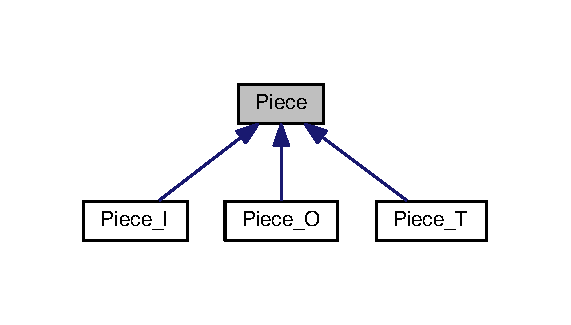
\includegraphics[width=274pt]{class_piece__inherit__graph}
\end{center}
\end{figure}
\subsection*{Public Member Functions}
\begin{DoxyCompactItemize}
\item 
\mbox{\Hypertarget{class_piece_a0af5276d26a4bb2a6a42a3dab8b4783f}\label{class_piece_a0af5276d26a4bb2a6a42a3dab8b4783f}} 
int {\bfseries get\+Posx} (int i) const
\item 
\mbox{\Hypertarget{class_piece_a24ca14604d394b821bf89d690c6de477}\label{class_piece_a24ca14604d394b821bf89d690c6de477}} 
int {\bfseries get\+Posy} (int i) const
\item 
\mbox{\Hypertarget{class_piece_a6a72e18613ea141e736c594b0440eac1}\label{class_piece_a6a72e18613ea141e736c594b0440eac1}} 
void {\bfseries set\+Posx} (int i, int j)
\item 
\mbox{\Hypertarget{class_piece_a4d7e79b948de16a1608d4cbf97f20b5e}\label{class_piece_a4d7e79b948de16a1608d4cbf97f20b5e}} 
void {\bfseries set\+Posy} (int i, int j)
\item 
\mbox{\Hypertarget{class_piece_aa5f13b2ce17fdf29dca28b0455f7b73a}\label{class_piece_aa5f13b2ce17fdf29dca28b0455f7b73a}} 
bool {\bfseries getbloque} ()
\item 
\mbox{\Hypertarget{class_piece_a2160d48bd04821ebbab32e14728360ad}\label{class_piece_a2160d48bd04821ebbab32e14728360ad}} 
int {\bfseries getcolor} ()
\item 
\mbox{\Hypertarget{class_piece_ad48708c0bbee0b0a583f00e56808b1d2}\label{class_piece_ad48708c0bbee0b0a583f00e56808b1d2}} 
bool {\bfseries Down} (\hyperlink{class_board}{Board} b)
\item 
\mbox{\Hypertarget{class_piece_aaef48eb5277927bcacace16aaf2d9636}\label{class_piece_aaef48eb5277927bcacace16aaf2d9636}} 
bool {\bfseries Left} (\hyperlink{class_board}{Board} b)
\item 
\mbox{\Hypertarget{class_piece_a44d684a99ea99db740b5bfa73f37ab15}\label{class_piece_a44d684a99ea99db740b5bfa73f37ab15}} 
bool {\bfseries Right} (\hyperlink{class_board}{Board} b)
\item 
\mbox{\Hypertarget{class_piece_a44530e200e9506f7bb4668e82dd91d54}\label{class_piece_a44530e200e9506f7bb4668e82dd91d54}} 
void {\bfseries Move\+Down} (\hyperlink{class_board}{Board} b)
\item 
\mbox{\Hypertarget{class_piece_a938328bd15662dbf8d4bd66145e20e1a}\label{class_piece_a938328bd15662dbf8d4bd66145e20e1a}} 
void {\bfseries Move\+Right} (\hyperlink{class_board}{Board} b)
\item 
\mbox{\Hypertarget{class_piece_a08f2bd761965092bd4f8f97c81aa6af8}\label{class_piece_a08f2bd761965092bd4f8f97c81aa6af8}} 
void {\bfseries Move\+Left} (\hyperlink{class_board}{Board} b)
\item 
\mbox{\Hypertarget{class_piece_aec441d76f79402f908b60c84abd7d998}\label{class_piece_aec441d76f79402f908b60c84abd7d998}} 
virtual void {\bfseries Rotate} (\hyperlink{class_board}{Board} b)=0
\item 
\mbox{\Hypertarget{class_piece_a9a74ccee356f6587b48befeed98f1ca1}\label{class_piece_a9a74ccee356f6587b48befeed98f1ca1}} 
virtual bool {\bfseries is\+Rotateable} (\hyperlink{class_board}{Board} b)=0
\end{DoxyCompactItemize}
\subsection*{Protected Attributes}
\begin{DoxyCompactItemize}
\item 
\mbox{\Hypertarget{class_piece_a9ea65e906b9ef0c30594f4f5aa5ed444}\label{class_piece_a9ea65e906b9ef0c30594f4f5aa5ed444}} 
vector$<$ \hyperlink{class_bloc}{Bloc} $>$ {\bfseries tab}
\item 
\mbox{\Hypertarget{class_piece_a9632e25aa0e79f8161451a937ccfc7ad}\label{class_piece_a9632e25aa0e79f8161451a937ccfc7ad}} 
int {\bfseries etat}
\item 
\mbox{\Hypertarget{class_piece_a99b4e2bbf91e0e609fc5141135a2e0ad}\label{class_piece_a99b4e2bbf91e0e609fc5141135a2e0ad}} 
bool {\bfseries bloque}
\item 
\mbox{\Hypertarget{class_piece_a4268f3b047e1ad284882708b85332ef1}\label{class_piece_a4268f3b047e1ad284882708b85332ef1}} 
int {\bfseries color}
\item 
\mbox{\Hypertarget{class_piece_af0c815c20f2000c02b6d7ce5b6703651}\label{class_piece_af0c815c20f2000c02b6d7ce5b6703651}} 
bool {\bfseries stocke}
\end{DoxyCompactItemize}


The documentation for this class was generated from the following files\+:\begin{DoxyCompactItemize}
\item 
Piece.\+hpp\item 
Piece.\+cpp\end{DoxyCompactItemize}

\hypertarget{class_piece___i}{}\section{Piece\+\_\+I Class Reference}
\label{class_piece___i}\index{Piece\+\_\+I@{Piece\+\_\+I}}


Inheritance diagram for Piece\+\_\+I\+:
\nopagebreak
\begin{figure}[H]
\begin{center}
\leavevmode
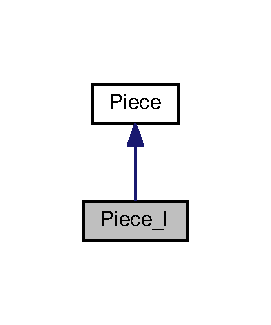
\includegraphics[width=130pt]{class_piece___i__inherit__graph}
\end{center}
\end{figure}


Collaboration diagram for Piece\+\_\+I\+:
\nopagebreak
\begin{figure}[H]
\begin{center}
\leavevmode
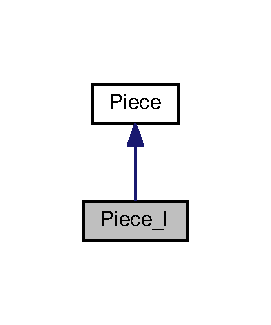
\includegraphics[width=130pt]{class_piece___i__coll__graph}
\end{center}
\end{figure}
\subsection*{Public Member Functions}
\begin{DoxyCompactItemize}
\item 
\mbox{\Hypertarget{class_piece___i_aec103ce64d2702bf3dc5dbcdb8b450eb}\label{class_piece___i_aec103ce64d2702bf3dc5dbcdb8b450eb}} 
virtual bool {\bfseries is\+Rotateable} (\hyperlink{class_board}{Board} b)
\item 
\mbox{\Hypertarget{class_piece___i_ab7983a575f6d5d41cbf846b6240a9b43}\label{class_piece___i_ab7983a575f6d5d41cbf846b6240a9b43}} 
virtual void {\bfseries Rotate} (\hyperlink{class_board}{Board} b)
\end{DoxyCompactItemize}
\subsection*{Additional Inherited Members}


The documentation for this class was generated from the following files\+:\begin{DoxyCompactItemize}
\item 
Piece\+\_\+\+I.\+hpp\item 
Piece\+\_\+\+I.\+cpp\end{DoxyCompactItemize}

\hypertarget{class_piece___o}{}\section{Piece\+\_\+O Class Reference}
\label{class_piece___o}\index{Piece\+\_\+O@{Piece\+\_\+O}}


Inheritance diagram for Piece\+\_\+O\+:
\nopagebreak
\begin{figure}[H]
\begin{center}
\leavevmode
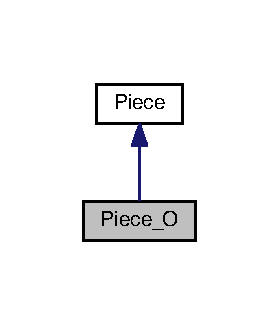
\includegraphics[width=134pt]{class_piece___o__inherit__graph}
\end{center}
\end{figure}


Collaboration diagram for Piece\+\_\+O\+:
\nopagebreak
\begin{figure}[H]
\begin{center}
\leavevmode
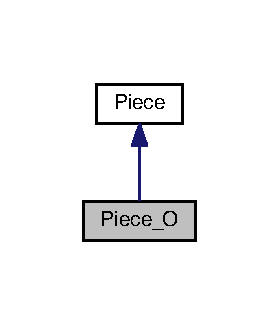
\includegraphics[width=134pt]{class_piece___o__coll__graph}
\end{center}
\end{figure}
\subsection*{Public Member Functions}
\begin{DoxyCompactItemize}
\item 
\mbox{\Hypertarget{class_piece___o_af82900ecec4e7bd058d43825293d8bff}\label{class_piece___o_af82900ecec4e7bd058d43825293d8bff}} 
bool {\bfseries is\+Rotateable} (\hyperlink{class_board}{Board} b)
\item 
\mbox{\Hypertarget{class_piece___o_a69812f938582f176cd4cca997cbb87c1}\label{class_piece___o_a69812f938582f176cd4cca997cbb87c1}} 
void {\bfseries Rotate} (\hyperlink{class_board}{Board} b)
\end{DoxyCompactItemize}
\subsection*{Additional Inherited Members}


The documentation for this class was generated from the following files\+:\begin{DoxyCompactItemize}
\item 
Piece\+\_\+\+O.\+hpp\item 
Piece\+\_\+\+O.\+cpp\end{DoxyCompactItemize}

\hypertarget{class_piece___t}{}\section{Piece\+\_\+T Class Reference}
\label{class_piece___t}\index{Piece\+\_\+T@{Piece\+\_\+T}}


Inheritance diagram for Piece\+\_\+T\+:
\nopagebreak
\begin{figure}[H]
\begin{center}
\leavevmode
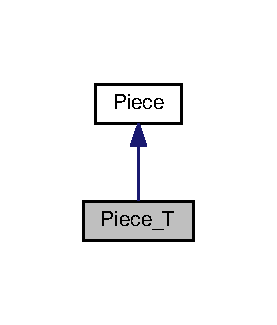
\includegraphics[width=133pt]{class_piece___t__inherit__graph}
\end{center}
\end{figure}


Collaboration diagram for Piece\+\_\+T\+:
\nopagebreak
\begin{figure}[H]
\begin{center}
\leavevmode
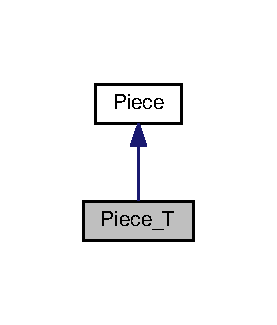
\includegraphics[width=133pt]{class_piece___t__coll__graph}
\end{center}
\end{figure}
\subsection*{Public Member Functions}
\begin{DoxyCompactItemize}
\item 
\mbox{\Hypertarget{class_piece___t_a64088f0140b870d178169e36460cd4de}\label{class_piece___t_a64088f0140b870d178169e36460cd4de}} 
bool {\bfseries is\+Rotateable} (\hyperlink{class_board}{Board} b)
\item 
\mbox{\Hypertarget{class_piece___t_affedcbe550aebd2a9e8ec169d1fe0a9f}\label{class_piece___t_affedcbe550aebd2a9e8ec169d1fe0a9f}} 
void {\bfseries Rotate} (\hyperlink{class_board}{Board} b)
\end{DoxyCompactItemize}
\subsection*{Additional Inherited Members}


The documentation for this class was generated from the following files\+:\begin{DoxyCompactItemize}
\item 
Piece\+\_\+\+T.\+hpp\item 
Piece\+\_\+\+T.\+cpp\end{DoxyCompactItemize}

%--- End generated contents ---

% Index
\backmatter
\newpage
\phantomsection
\clearemptydoublepage
\addcontentsline{toc}{chapter}{Index}
\printindex

\end{document}
